%!TEX root = main.tex
%%%%%%%%%%%%%%%%%%%%%%%%%%%%%%%%%%%%%%%%%%%%%%%%%%%%%%%%%%%%%%%%%%%%%%%%%%%%%%%%%%%%%%%%%%%%%%%%%%%%%%
%
%   Filename    : chapter_1.tex 
%
%   Description : This file will contain your Research Description.
%                 
%%%%%%%%%%%%%%%%%%%%%%%%%%%%%%%%%%%%%%%%%%%%%%%%%%%%%%%%%%%%%%%%%%%%%%%%%%%%%%%%%%%%%%%%%%%%%%%%%%%%%%

%% ==== Notes from Sir JD: Please answer the questions I'll be putting here



%added by sir jd just for fun
\epigraph{Music is a science which must have determined rules. These rules must be drawn from a principle which should be evident, and this principle cannot be known without the help of mathematics. I must confess that in spite of all the experience which I have acquired in music by practicing it for a fairly long period, it is nevertheless only with the help of mathematics that my ideas became disentangled and that light has succeeded to a certain darkness of which I was not aware before.}{\textit{\citet{rameau1722traite}}}
\chapter{Research Description}
\label{sec:researchdesc}    %--note: labels help you with hyperlink editing (using your IDE)

This chapter is composed of the introduction, overview of the current state of musical metacreation, the research problem, objectives, scope, limitations and significance. The motivation behind the study will also be discussed in this chapter. 

\section{Overview of the Current State of Technology}
\label{sec:overview}
%
%   ==== The Overview of the Current State of Technology should usually contain three main paragraphs that ends with the problem at hand. The last few sentences of this section should be a problematic statement that rougly introduces the reader to the statement of the problem. 
%

%%=== begin with: describing the process of musical composition, then proceed with the what technologies, in summary, have been crafted to assist the musical composition process.

The discipline of composing music can be traced to as far back as ancient Greece \citep{burney1789general}. It is a specific and careful craft that requires many characteristics such as discipline, skill and immense patience. The approach of composing music itself has given birth to newer genres and sub-genres as composers have grown more creative and personal with their creations \citep{miller1984genre}. Some composers even follow a strict set of theories and guidelines to maintain the aesthetic quality of the music they create \citep{rothgeb1975strict,collins2005synthesis}. 

% Discuss composition here
% Music composition goes through multiple stages containing factors that composers have described as both spontaneous and deliberate \citep{bennett1976process}. This process, illustrated in Figure \ref{fig:composing-graph}, begins with the idea of a melody or harmony culminating into a final draft of the musical piece and undergoing revisions if necessary.

% Composers traverse through these stages with different dispositions and actions that will eventually lead them to the completion of their musical piece but a similarity can be found among a majority of composers. Composers are sensitive to the input they receive from the environment they are in while processing or looking for the idea of their piece \citep{bennett1976process}. Once the idea has come to fruition, a composer will lay down the foundations of the musical piece which will come from their knowledge in music \citep{graf2013beethoven}. When the foundations are in place, and the composer has a rough framework of the piece, only then will it be tested and completed through careful composing \citep{graf2013beethoven}. However, the process is usually repeated as musical composition is a trial-and-error process and requires experimentation \citep{macdonald2006creativity}. Even for experts, music composition can still be a daunting task \citep{kikuchi2016music}.

Music composition goes through multiple stages containing factors that composers have described as both spontaneous and deliberate \citep{bennett1976process}. This process is illustrated in Figure \ref{fig:composing-graph}. Composers traverse these stages with different methods and actions. But generally, musical composition begins with an initial idea that undergoes several revisions until it culminates into the final draft. However, this usually takes time as musical composition requires trial-and-error and requires experimentation \citep{gartland2003suitability, macdonald2006creativity}. Even for experts, music composition can still be a daunting task \citep{kikuchi2016music}.

% Composers are sensitive to the input they receive from the environment they are in while processing or looking for the idea of their piece \citep{bennett1976process}. Once the idea has come to fruition, a composer will lay down the foundations of the musical piece which will come from their knowledge in music \citep{graf2013beethoven}. When the foundations are in place, and the composer has a rough framework of the piece, only then will it be tested and completed through careful composing \citep{graf2013beethoven}. However, the process is usually repeated as musical composition is a trial-and-error process and requires experimentation \citep{macdonald2006creativity}. Even for experts, music composition can still be a daunting task \citep{kikuchi2016music}.


\begin{figure}[H]
    \centering
	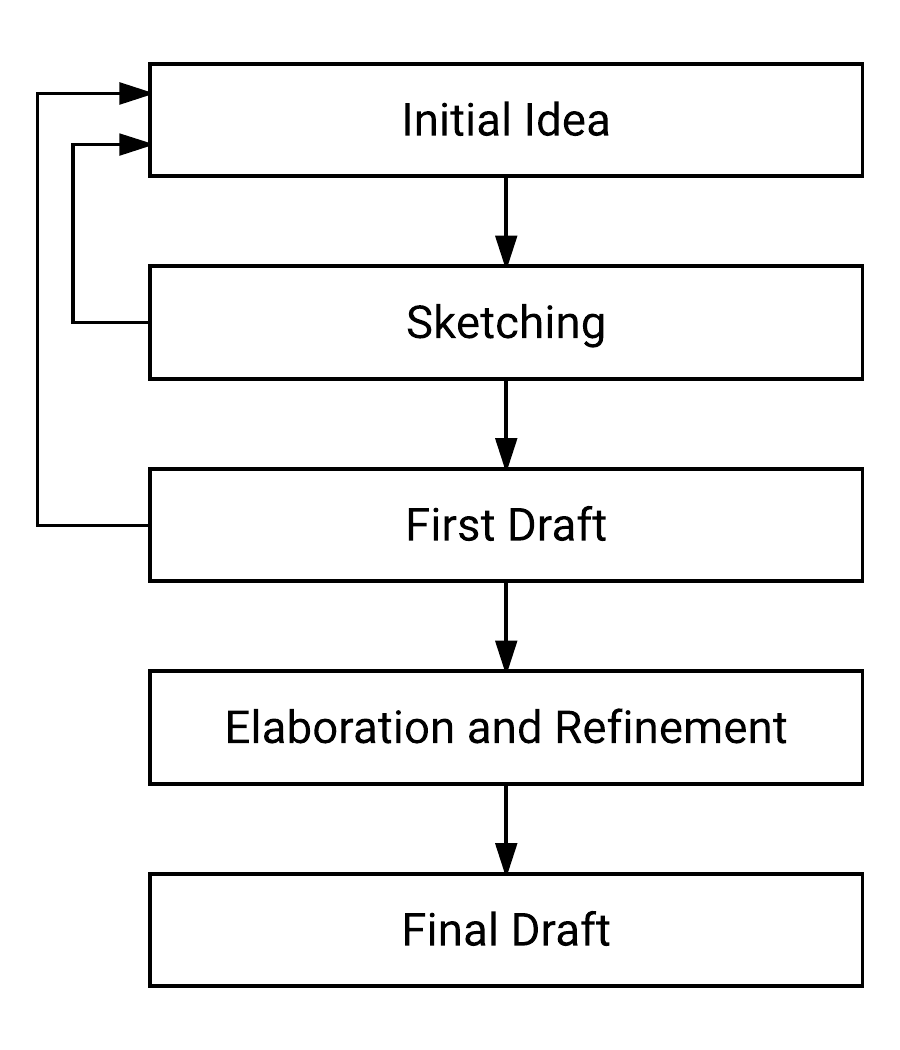
\includegraphics[scale=0.2]{Process_of_Composition}
    \caption{The stages of music composition \citep{bennett1976process}.}
    \label{fig:composing-graph}
\end{figure}

%%need to add gestures in the overview more to define the thingy use of UX in conjunction with the music composition process

There have been several attempts to ease the drafting phase's repetitiveness. To solve this problem, composers along with computer scientists have looked towards \textit{musical metacreation}. This subfield of computational creativity is focused on granting machines the creative capacity to perform musical tasks like composition \citep{pasquier2017an}.

One example of metacreation is found in the case of MorpheuS \citep{herremans2016morpheus}, a music generation system that uses pattern detection techniques to generate music. Alternatively, \citet{kikuchi2016music} attempted to create a music composition tool with recommendations. They utilized gesture interactions, which are methods of communication with computers that use the fingers or hands to execute commands on a touchscreen device \citep{kammer2010towards}. Touch gestures were noted to be a possible medium in the communication of a composer and the computer in the field of music composition \citep{kurtenbach1996gestures}. The tool recommended succeeding notes based on the input provided by the user. 

%% === next main thought should be: given these technologies, what have been the gaps, difficulties encountered as you have seen in the literature???

However, despite these recent advancements, limitations are still present in the existing technologies. In the work of \citet{herremans2016morpheus}, it was admitted that MorpheuS still lacked in terms of musical output and efficiency. The music composition tool created in the study of \citet{kikuchi2016music} was dependent on an existing musical composition because it extracted the rules such as pitch transition and rhythm to predict eventual notes, not from the known strict musical guidelines. This process led to a lack of variety in the generated musical compositions.

\begin{comment}
To solve this lack of variety there were studies that focused on generating musical structures that adhere to a specific theme. Some researchers focused on the structure of happy melodies where they discerned the emotion of happiness in the algorithm by defining explicit rules and using relations to form a generated theme phrase \citep{cao2015automatic}. It was also noted that the researchers created variance in the system by adding a factor of randomness in the pitch generation while still keeping true to the theme of happiness \citep{cao2015automatic}. This yielded computer generated music that was comparable to man-made music \citep{cao2015automatic}.
\end{comment}

Additional studies that desired for computer generated music to be less ``robotic'' focused on the expressive trait of a performer through various elements like emotion \citep{bresin2000emotional}, imitation \citep{miranda2010artificial}, and selection \citep{ramirez2008genetic}. One such study focused on the structure of happy melodies where they discerned the emotion of happiness in the algorithm by defining explicit rules and using relations to form a generated theme phrase \citep{cao2015automatic}. It was also noted that the researchers created variance in the system by adding a factor of randomness in the pitch generation while still keeping true to the theme of happiness \citep{cao2015automatic}. 

From the various algorithms available, most can generate expressive music based on their evaluation metrics \citep{cao2015automatic,bresin2000emotional,miranda2010artificial,de2012playing,ramirez2008genetic,miranda2010artificial} but lacked a usable interface for composers. Computers can help increase the productivity of composers by aiding them during musical composition \citep{velardo2016study}. One such system is Computoser which provided the user with a form based interface that generated music based on choices from multiple selections, and a probability and rule-based algorithm \citep{bozhanov2014computoser}. 

Similar to previous systems, Computoser takes in training data and performs a machine learning algorithm to generate a metacreation model. It was deployed on a website for ease-of-access. However, the interface is form-based and limits the possible compositions (see Figure \ref{fig:computoser-preference}). 

\begin{comment}
One such tool is the Abjad API, an open source software for Python. The tool assists users in creating a musical score by expanding the Python programming language with additional functions that can be used in Python programs \citep{baca2015abjad}. Despite its availability, the tool can only be used by users knowledgeable in the Python programming language and is inaccessible to composers who cannot code. To open computational creativity into a wider audience of composers, there is a need to have a usable interface that does not require any knowledge other than a general understanding of music composition.
\end{comment}

\begin{figure}[H]
    \centering
	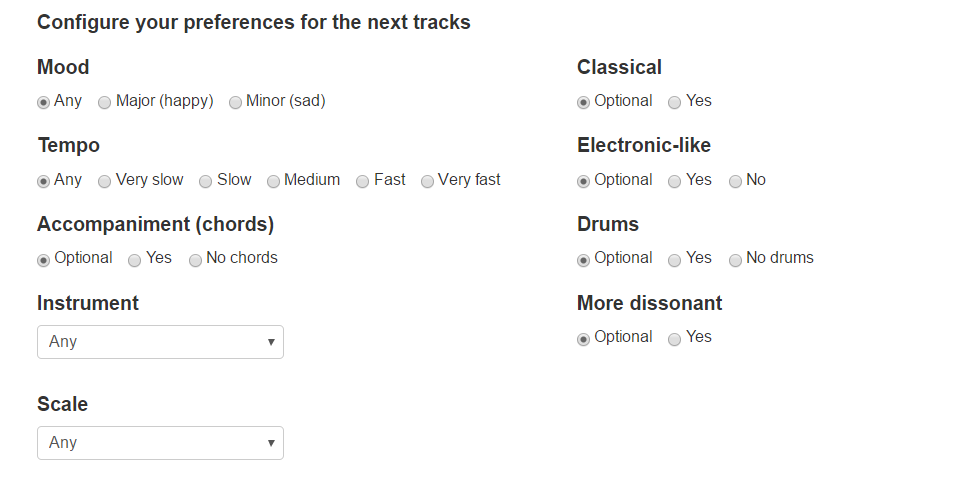
\includegraphics[scale=0.7]{ComputoserSelectionForm}
    \caption{\textit{Computoser} preference selection form \citep{bozhanov2014computoser}.}
    \label{fig:computoser-preference}
\end{figure}

%% === the last main thought of this section should be, summarizing and leading to the research problem that we all intended to solve


The underlying case behind all these findings is figuring out how existing studies on human-computer interactions may augment the current process of music composition. It was found by \citet{brown2017user} that the user experience component was often overlooked when designing interfaces aimed at enhancing the musical composition process. It was suggested in the study of \citep{levitt1992representation} that a computer ``assistant'' that helps the composer during creative lapses would be more beneficial than a system that automatically composes music without any control provided to the user. 

Numerous works on musical metacreation have focused on the algorithms related to music generation and there are limited studies that explore the utilization of human-computer interaction to augment the musical composition process.

\begin{comment}
Although there are already several musical composition tools that aid in the composition of music such as Hyperscore \citep{farbood2004hyperscore} and HARP \citep{camurri1991harp}, the ability to assist composers in a way that it helps them generate ideas are what these systems lack. The graphical user interface of these systems improve the overall user experience of musical composers, but the important problem still remains which is coming up with musical ideas. 
\end{comment}


%% === However, there are possible methods to increase the diversity of the generated music to achieve a level of variety that can be seen as 
   

\section{Research Objectives}
\label{sec:researchobjectives}

\subsection{General Objective}
\label{sec:generalobjective}

To augment the musical composition process by integrating rule-based musical metacreation and gesture interactions

\subsection{Specific Objectives}
\label{sec:specificobjectives}

\begin{enumerate}
	\item To design and develop an application that users can utilize for basic musical composition tasks
    \item To design interactions that will enable users to perform advanced musical composition tasks
    \item To assign gesture interactions for doing compositional tasks in a mobile composition tool
    \item To validate whether the interaction design improves the user experience when using the tool

\end{enumerate}

\section{Scope and Limitations of the Research}
\label{sec:scopelimitations}

The application will be developed for a mobile platform. Through the application, composers can perform basic composition tasks. This includes creating a composition, adding notes, editing notes, and deleting notes. The target instrument of the tool for composition is the piano, due to its popularity.

Only certain musical notation symbols will be available for use in the system. The minimum requirement is to allow composers to perform basic musical notation on a mobile interface.

Composers may perform advanced compositional tasks such as musical metacreation and note transposition. Additionally, composers may also edit multiple notes at the same time by highlighting them. The musical metacreation model will also be limited to a rule-based model.

Given that the application is on a mobile platform, the interactions will be limited to multi-touch gestures that can be handled by this platform. Examples of these gestures are tap, swipe, and flick gestures. The interface will be designed to support finger taps, but a stylus may also be used.

The system aims to provide a dynamic and interactive musical composition experience. To achieve this, it is important that the system's interaction design is tested on actual composers while they accomplish compositional tasks. The target users and testers are composers who have basic knowledge in writing sheet music. These are people who can read and write in musical notation for instrumental music, regardless of the platform or tool. Users are categorized into two (2) levels: newbie, and experienced. Testing will be done with at least 3 composers per level. However, due to the possible schedule limitations of experienced composers, testing with them will be saved for the latter parts of the research when the system has been polished through several iterations of testing. Additionally, to prevent bias, fresh users will be introduced during some iterations of testing. 

The main goal of the proposed solution is not to improve the quality of music produced by the composers, but to aid them in their composition process. It would not replace the composers, as it would only provide suggestions based on the input given by the composer. It is up to the discretion of the composer whether or not to use the metacreated music.

\section{Significance of the Research}
\label{sec:significance}

This study will produce an accessible musical composition tool incorporating concepts from both musical metacreation and human-computer interaction. Given that there are limited studies that use rule-based models, this study will contribute to the emerging field of computational creativity and musical metacreation.

Additionally, the function of the tool will be to augment the musical composition experience of composers. Concepts from both human-computer interaction and music theory will be integrated into the tool to achieve this. Findings from this study will contribute to the knowledge on the process of musical composition, and will provide a background on the integration of human-computer interaction in musical composition.

With the developed system, the improved user experience will help the composer focus more on the composition and the output rather than operating the tool. This would benefit composers that experience creative blocks or have an initial melody in mind, but have no idea how to continue. The tool will aid composers to create music that will still reflect their own style. The personal style of a composer is formed by the culture of the composer. The music created by every composer may reflect their cultural background and personal experiences. This will result in a composition that is a product of an augmented experience but still fully the work of the composer.

Lastly, it is widely known that music has made a great impact on society through the entertainment it brings to people \citep{hawkins2013pac, donnelly2005spectre} and also its therapeutic benefits in common psychological disorders \citep{kemper2005music}. Helping make the composition easier for composers regardless of skill level would allow for better access to music and thereby also granting benefits to society through the several uses of music.

% May problem ako with adding the paradigm of adding focus to Filipino Composers kasi baka mahihirapan tayo mag dagdag pa ng stuff for that, halos lahat ng chapters madadagdagan kapag minention ko Filipino composers dito. Hahanapan nila ng extra proof kung bakit yung tool natin mas makakatulong sa Filipino Composers opposed to other composers

\section{Research Methodology}
This chapter lists and discusses the specific steps and activities that will be performed by the proponent to accomplish the project. 
The discussion covers the activities from pre-proposal to Final Thesis Writing.  It also includes an initial discussion on the theoretical
framework to be followed.

\subsection{Research Activities}

\subsubsection{Planning}
This phase concerns the whole group, with the guidance of the thesis adviser. It involves the formulation of the thesis topic, including the research problem, research objectives, as well as the scope and limitations. This would also include the planning on the approach, and desired output of the study. 

\subsubsection{Review of Related Literature}
Relevant works on musical metacreation, musical composition, and gesture interactions are being studied and synthesized by the group to provide context, and the necessary understanding to perform the study. Works related to musical metacreation are essential to the study due to the insight they provide on how past works have attempted to generate music through different algorithms and modalities. Works on musical composition will be reviewed because they provide a background on the musical theories, as well as the attempts made to augment the musical composition process. Finally, works on gesture interactions will also be reviewed to give context on how gestures play an important role in human-computer interaction as well as how past studies have implemented and studied the said technology in relation to the musical composition process.

\subsubsection{Data Collection}
The group will be doing two kinds of data collection. The first one involves research on music theory and the chord progressions present in music. The information gathered on this will be used for building the model for the system. For the second kind of data, at least three (3) composers will be interviewed to gather data on the musical composition process. Being a study related to human-computer interaction, it is essential that the group understand more about how composers compose music in order to design good interactions to augment the process. Interviews will mainly be done face-to-face, with questions focused on how the composer composes music. Specific details like how the composer transitions from testing a melody to writing it digitally or on paper will be observed. Finally, the composer will also be asked to validate or test a prototype of the proposed system. However before interviews, they will be provided a consent form that would explain what to expect in the interview and testing. They are given the freedom to cancel the interview if they choose to. This will mainly be conducted in the School of Design and Arts building in the De La Salle-College of Saint Benilde. However, depending on the availability of the composers, interviews may also be done in other locations. 

\subsubsection{Interaction Design}
This phase involves design thinking, as it is concerned with the application's user experience and how it would benefit the target users. Interaction design would also include identifying the right placement of user interface (UI) elements, as well as the right methods to interact with them (i.e. gestures and taps). The data gathered from the observations and interviews with composers would provide the insight necessary to make design decisions that would result in an interaction that benefits the users. Design artifacts like affinity diagrams and user personas would be used to represent these users in a collected, yet organized form. This will be done repeatedly, and will be validated through more interviews and tests. This is to ensure that the proposed solution would integrate seamlessly with the musical composition process.

% This phase is all about design thinking. It is concerned with the user experience design of the solution and how it can benefit the target users, composers. The data gathered during data collection, specifically the interviews with the composers, will be maximized in this phase since it would provide the insight necessary to understand how they compose. This will be done repeatedly, with validation, to ensure that the solution will integrate seamlessly with the musical composition process.

\subsubsection{Implementation}
Once the interaction design has been laid out and validated, the actual system can then be implemented. The system will be in the form of a mobile application in the iOS platform. It will be optimized for iPads, due to its larger screen size compared to regular phones. The validated interaction design formulated during the previous phase would be implemented in the application. This phase would involve iterations of more testing and development to continuously gather user experience and interaction data that would help improve the application's design.

% Included in this phase will be the necessary testing in order to ensure the model's correctness, accuracy, and usability.

\subsubsection{Experiment Design}
 In order to assess the effectiveness of the developed system, experiments will have to be conducted in every iteration throughout the study. However, these experiments have to be designed so that they could effectively measure interaction and user experience. With that said, common user experience metrics like KLM-GOMS, and Fitts Law will be used and measured using CogTool. Additionally, testing will be done with at least two (2) experienced and three (3) amateur composers, totaling to at least five (5) composers. Before the testing, they will be given a consent form indicating the ethical considerations of the research. At this point, they may choose to opt out of the testing or continue with it. If they continue, they will be asked to perform a set of tasks that would help the researchers identify any flaws or issues that can be improved in the user experience and interaction design. Note that these composers may change in between iterations to prevent bias and inaccurate results. 

% In order to assess the effectiveness of the developed system, experiments will have to be conducted throughout the course of this study. However, in order for the results to be as accurate as possible, the experiments have to be designed accordingly so that they measure interaction and user experience. Research will be done on how to effectively measure user experience metrics and system interaction. This will involve creating use cases, test scenarios, and identifying the pains and gains of the users. Testing will be done with at least three (3) composers per level (newbie and experienced), totaling to at least six (6) composers. Before the testing, they will be given a consent form indicating the ethical considerations of the research. At this point, they may choose to opt out of the testing, or continue with it. 

\subsubsection{Results Analysis}
This activity will include analysis on the findings gathered during review of related literature, data collection, and experimentation. It involves performing quantitative and/or qualitative analyses on the gathered data and review them in order to improve the system. This will also involve creating use cases, test scenarios, and identifying the pains and gains of the users. The privacy of the respondents will also be maintained, with any information about them including their name, age, or working experience hidden. Any results or comments received from the users will only be used for this study. They will not be released or publicized in any form. The researchers will be implementing a methodology called \textit{user personas} to represent users without having to compromise their privacy.

\subsubsection{Documentation}
The documentation will be done during the entire study. This will include documentation on all the activities performed, as well as their results and discussion.

\subsection{Calendar of Activities}
Table \ref{tab:timetableactivities} shows a Gantt chart of the activities.  Each bullet represents approximately
one week worth of activity.

%
%  the following commands will be used for filling up the bullets in the Gantt chart
%
\newcommand{\weekone}{\textbullet}
\newcommand{\weektwo}{\textbullet \textbullet}
\newcommand{\weekthree}{\textbullet \textbullet \textbullet}
\newcommand{\weekfour}{\textbullet \textbullet \textbullet \textbullet}

%
%  alternative to bullet is a star 
%
\begin{comment}
   \newcommand{\weekone}{$\star$}
   \newcommand{\weektwo}{$\star \star$}
   \newcommand{\weekthree}{$\star \star \star$}
   \newcommand{\weekfour}{$\star \star \star \star$ }
\end{comment}

\begin{comment}
\begin{table}[ht]  %t means place on top, replace with b if you want to place at the bottom
\centering
\caption{Timetable of Activities} \vspace{0.25em}
\begin{tabular}{|p{2in}|c|c|c|c|c|c|c|c|c|} \hline
\centering Activities-2017 & May & Jun & Jul & Aug & Sep & Oct & Nov & Dec \\ \hline
Planning     & ~~\weekone~ & \weekone~~~ & \weekone~~~ & \weekone~~~ & & & & \\ \hline
Review of Related Literature & ~~\weektwo & \weekfour & \weekfour & \weekone~~~ &  &  & & \\ \hline
Data Collection     &   &  & ~~~\weekone & \weekfour & \weekone~~~ &  &  &\\ \hline
Interaction Design    &   &  &  & \weekfour & \weektwo~~ &  &&  \\ \hline
Implementation      &   &  &  &  & \weekfour & \weekfour & \weektwo~~ &\\ \hline
Experiment Design &   &  &  &  &  & ~~\weektwo & \weekfour & \\ \hline
Results Analysis &  &  &  &  & & &  & \weektwo~~ \\ \hline
Documentation & ~~~\weekone  & ~~~\weekone & ~~~\weekone & ~~~\weekone & ~~~\weekone & ~~~\weekone & ~~~\weekone & \weekone~~~ \\ \hline
\end{tabular}
\label{tab:timetableactivities}
\end{table}

\begin{table}[ht]  %t means place on top, replace with b if you want to place at the bottom
\centering
\begin{tabular}{|p{2in}|c|c|c|c|c|c|c|c|c|} \hline
\centering Activities-2018 & Jan & Feb & Mar & April & May & Jun & Jul & Aug \\ \hline
Planning     & ~\weekone~~  & \weekone~~ &  &  & \weekone &  &  & \\ \hline
Review of Related Literature &  & & & ~~\weektwo & \weektwo~~ & & & \\ \hline
Data Collection     &   &  &  & & &  &  &\\ \hline
Interaction Design    &  & \weekfour & \weekfour & & &  &&  \\ \hline
Implementation      &   &  & \weekfour & \weekfour &  & &  &\\ \hline
Experiment Design &   &  &  & \weekfour & \weektwo~~ &  & & \\ \hline
Results Analysis & ~\weekthree & \weekfour & &  & \weekfour & \weekfour &  &  \\ \hline
Documentation & ~~~\weekone  & ~~~\weekone & ~~~\weekone & ~~~\weekone & ~~~\weekone & ~~~\weekone & \weekfour & \weektwo~~ \\ \hline
\end{tabular}
\label{tab:timetableactivities2}
\end{table}
\end{comment}

\begin{landscape} % Landscape page
\begin{table} [!htbp]  
\centering
\caption{Timetable of Activities} \vspace{0.25em}
\begin{tabular}{|p{1.1in}|c|c|c|c|c|c|c|c|c|c|c|c|c|c|c|c|c|} \hline
  \centering 2017-2018 & May & Jun & Jul & Aug & Sep & Oct & Nov & Dec & Jan & Feb & Mar & Apr & May & Jun & Jul\\ \hline
  Planning     & ~~\weekone~ & \weekone~~~ & \weekone~~~ & \weekone~~~ & & & & & ~\weekone~~  & \weekone~~ &  &  & \weekone &  & \\ \hline
  Review of Related Literature & ~~\weektwo & \weekfour & \weekfour & \weekone~~~ &  &  & & &  & & & ~~\weektwo & \weektwo~~ & & \\ \hline
  Data Collection     &   &  & ~~~\weekone & \weekfour & \weekone~~~ &  &  & &   &  &  & & &  &  \\ \hline
  Interaction Design    &   &  &  & \weekfour & \weektwo~~ &  & &  &  & \weekfour & \weekfour & & &  & \\ \hline
  Implementation      &   &  &  &  & \weekfour & \weekfour & \weektwo~~ & &   &  & \weekfour & \weekfour &  & &  \\ \hline
  Experiment Design &   &  &  &  &  & ~~\weektwo & \weekfour & &   &  &  & \weekfour & \weektwo~~ &  & \\ \hline
  Results Analysis &  &  &  &  & & &  & \weektwo~~ & ~\weekthree & \weekfour & &  & \weekfour & \weekfour & \\ \hline
  Documentation & ~~~\weekone  & ~~~\weekone & ~~~\weekone & ~~~\weekone & ~~~\weekone & ~~~\weekone & ~~~\weekone & \weekone~~~ & ~~~\weekone  & ~~~\weekone & ~~~\weekone & ~~~\weekone & ~~\weektwo & \weekfour & \weekfour\\ \hline
\end{tabular}
\label{tab:timetableactivities}
\end{table}
\end{landscape}



